\section*{Entities}

The chosen area of the databases basics learning is the research about how different factors influence on the students education progress. Entities, forming the chosen area are described below.

\subsection*{Student}

This entity includes some personal information about current student. There are attributes which describes the entity:

\begin{figure}[H]
    \centering
    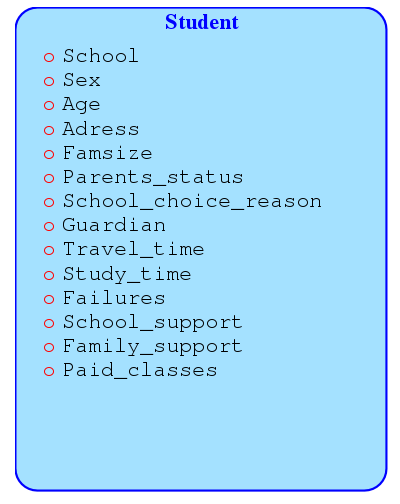
\includegraphics[width=0.75\textwidth]{Student.png}
    \caption{Student entity}
\end{figure}

\begin{enumerate}
\item \textbf{School} -- student's school (binary: 'GP' - Gabriel Pereira or 'MS' - Mousinho da Silveira). \textbf{Data type} -- text.
\item \textbf{Sex} -- student's sex (binary: 'F' - female or 'M' - male). \textbf{Data type} -- text.
\item \textbf{Age} -- student's school (binary: 'GP' - Gabriel Pereira or 'MS' - Mousinho da Silveira). \textbf{Data type} -- numeric.
\item \textbf{Adress} -- student's home address type (binary: 'U' - urban or 'R' - rural)  . \textbf{Data type} -- text.
\item \textbf{Famsize} -- family size (binary: 'LE3' - less or equal to 3 or 'GT3' - greater than 3). \textbf{Data type} -- text.
\item \textbf{Parents\_status} -- parent's cohabitation status (binary: 'T' -- living together or 'A' -- apart). \textbf{Data type} -- text.
\item \textbf{School\_choice\_reason} -- reason to choose this school (nominal: close to 'home', school 'reputation', 'course' preference or 'other') . \textbf{Data type} -- text.
\item \textbf{Guardian} -- student's guardian (nominal: 'mother', 'father' or 'other'). \textbf{Data type} -- text.
\item \textbf{Travel\_time} -- home to school travel time (numeric: 1 - <15 min., 2 - 15 to 30 min., 3 - 30 min. to 1 hour, or 4 - >1 hour). \textbf{Data type} -- numeric.
\item \textbf{Study\_time} -- weekly study time (numeric: 1 - <2 hours, 2 - 2 to 5 hours, 3 - 5 to 10 hours, or 4 - >10 hours). \textbf{Data type} -- numeric.
\item \textbf{Failures} -- number of past class failures (numeric: n if 1<=n<3, else 4). \textbf{Data type} -- numeric.
\item \textbf{School\_support} -- extra educational support (binary: yes or no). \textbf{Data type} -- boolean.
\item \textbf{Family\_support} -- family educational support (binary: yes or no). \textbf{Data type} -- boolean.
\item \textbf{Paid\_classes} -- extra paid classes within the course subject (Math or Portuguese) (binary: yes or no). \textbf{Data type} -- boolean.
\end{enumerate}

\subsection*{Social info}

This entity includes some additional information from the social poll.

\begin{figure}[H]
    \centering
    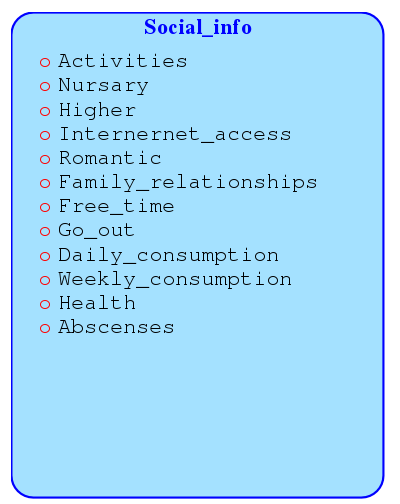
\includegraphics[width=0.75\textwidth]{Social.png}
    \caption{Social info entity}
\end{figure}

\begin{enumerate}
\item \textbf{Acticities} -- extra-curricular activities (binary: yes or no). \textbf{Data type} -- boolean.
\item \textbf{Nursary} -- attended nursery school (binary: yes or no). \textbf{Data type} -- boolean.
\item \textbf{Higher} -- wants to take higher education (binary: yes or no). \textbf{Data type} -- boolean.
\item \textbf{Internet\_access} -- Internet access at home (binary: yes or no). \textbf{Data type} -- boolean.
\item \textbf{Romantic} -- with a romantic relationship (binary: yes or no). \textbf{Data type} -- boolean.
\item \textbf{Family\_relationships} -- quality of family relationships (numeric: from 1 - very bad to 5 - excellent). \textbf{Data type} -- numeric.
\item \textbf{Free\_time} -- free time after school (numeric: from 1 - very low to 5 - very high). \textbf{Data type} -- numeric.
\item \textbf{Go\_out} -- going out with friends (numeric: from 1 - very low to 5 - very high). \textbf{Data type} -- numeric.
\item \textbf{Daily\_consumption} -- workday alcohol consumption (numeric: from 1 - very low to 5 - very high). \textbf{Data type} -- numeric.
\item \textbf{Weekend\_consumption} -- weekend alcohol consumption (numeric: from 1 - very low to 5 - very high). \textbf{Data type} -- numeric.
\item \textbf{Health} -- current health status (numeric: from 1 - very bad to 5 - very good). \textbf{Data type} -- numeric.
\item \textbf{Absences} -- number of school absences (numeric: from 0 to 93) -- numeric.
\end{enumerate}

\subsection*{Parents}

This entity includes some information about student's parents.

\begin{figure}[H]
    \centering
    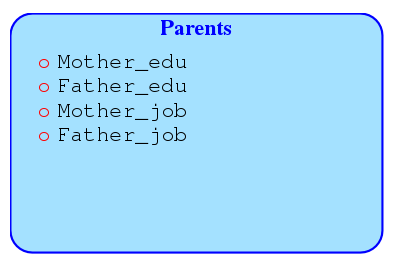
\includegraphics[width=0.75\textwidth]{Parents.png}
    \caption{Parents entity}
\end{figure}

\begin{enumerate}
\item \textbf{Mother\_edu} -- mother's education (numeric: 0 - none, 1 - primary education (4th grade), 2 – 5th to 9th grade, 3 – secondary education or 4 – higher education). \textbf{Data type} -- numeric.
\item \textbf{Father\_edu} -- father's education (numeric: 0 - none, 1 - primary education (4th grade), 2 – 5th to 9th grade, 3 – secondary education or 4 – higher education). \textbf{Data type} -- numeric.
\item \textbf{Mother\_job} -- mother's job (nominal: 'teacher', 'health' care related, civil 'services' (e.g. administrative or police), 'at home' or 'other'). \textbf{Data type} -- text.
\item \textbf{Father\_job} -- father's job (nominal: 'teacher', 'health' care related, civil 'services' (e.g. administrative or police), 'at home' or 'other'). \textbf{Data type} -- text.
\end{enumerate}

\subsection*{Scores}

This entity includes some information about student's scores.

\begin{figure}[H]
    \centering
    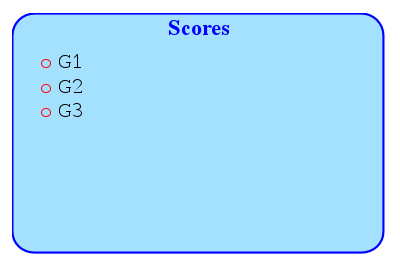
\includegraphics[width=0.75\textwidth]{Scores.png}
    \caption{Scores entity}
\end{figure}

\begin{enumerate}
\item \textbf{G1} -- first period grade (numeric: from 0 to 20). \textbf{Data type} -- numeric.
\item \textbf{G2} -- second period grade (numeric: from 0 to 20). \textbf{Data type} -- numeric.
\item \textbf{G3} -- last period grade (numeric: from 0 to 20). \textbf{Data type} -- numeric.
\end{enumerate}

\subsection*{Application}

This entity includes some information about student or parents applications.

\begin{figure}[H]
    \centering
    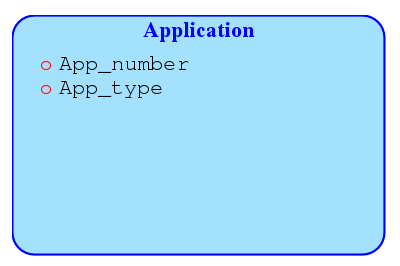
\includegraphics[width=0.75\textwidth]{Application.png}
    \caption{Application entity}
\end{figure}

\begin{enumerate}
\item \textbf{App\_number} -- The number of the application. \textbf{Data type} -- numeric.
\item \textbf{App\_type} -- The type of the application ('complaint' , 'request' ...). \textbf{Data type} -- text.
\end{enumerate}

\subsection*{Specialization}

This entity includes some information about student specialization.

\begin{figure}[H]
    \centering
    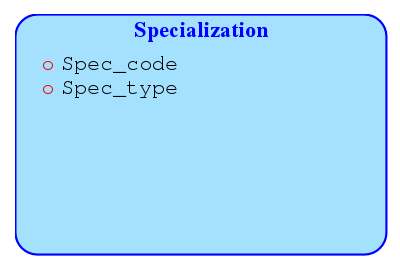
\includegraphics[width=0.75\textwidth]{Specialization.png}
    \caption{Specialization entity}
\end{figure}

\begin{enumerate}
\item \textbf{Spec\_code} -- The ID of the student specialization. \textbf{Data type} -- numeric.
\item \textbf{Spec\_type} -- The type of the specialization ('mathematical' , 'humanitarian' ...). \textbf{Data type} -- text.
\end{enumerate}

\subsection*{Subject}

This entity includes some information about subjects, learning by student.

\begin{figure}[H]
    \centering
    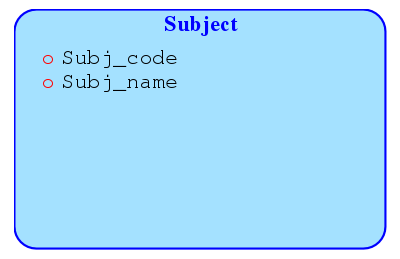
\includegraphics[width=0.75\textwidth]{Subject.png}
    \caption{Subject entity}
\end{figure}

\begin{enumerate}
\item \textbf{Subj\_code} -- The ID of the subject. \textbf{Data type} -- numeric.
\item \textbf{Subj\_name} -- The title of the subject ('maths' , 'physics' ...). \textbf{Data type} -- text.
\end{enumerate}